\documentclass{beamer}
\usetheme[sectionpage=progressbar, subsectionpage=progressbar, numbering=fraction, progressbar=foot, block=fill, background=light]{metropolis}
\usepackage{appendixnumberbeamer}
\usepackage{textpos}
\usepackage{booktabs}
\usepackage[scale=2]{ccicons}

\usepackage{pgfplots}
\usepgfplotslibrary{dateplot}
\usetikzlibrary{backgrounds}
\usepackage{xspace}
\newcommand{\themename}{\textbf{\textsc{metropolis}}\xspace}
\title{Attention based models in End-to-End ASR}
\subtitle{Exploration of Attention in ESPNET toolkit}
\date{\today}
\author{Shreekantha Nadig}
\institute{International Institute of Information Technology - Bangalore}
%\titlegraphic{\hfill\includegraphics[height=1.5cm]{logo.pdf}}

\usepackage{tikz}
\usetikzlibrary{shapes,shadows,arrows,patterns}

\tikzstyle{mlp} = [rectangle, draw, fill=blue!20, text width=5em, minimum height=5em, text centered, node distance=10em]
\tikzstyle{enc_h} = [rectangle, draw,  pattern=north west lines, pattern color=red!30, text width=1em, minimum height=10em, minimum width=3em, text centered, node distance=10em]
\tikzstyle{dec_z} = [rectangle, draw,  pattern=north east lines, pattern color=blue!30, text width=1em, minimum height=10em, minimum width=3em, text centered, node distance=10em]
\begin{document}
	\addtobeamertemplate{frametitle}{}{%
		\begin{textblock*}{100mm}(.97\textwidth,-1cm)
			{
\includegraphics[width=2.5em]{iiitb_logo.png}}
	\end{textblock*}}
	\maketitle

\begin{frame}{Table of contents}
	\setbeamertemplate{section in toc}[sections numbered]
	\tableofcontents[hideallsubsections]
\end{frame}


\begin{frame}[fragile]{test}
\begin{center}
	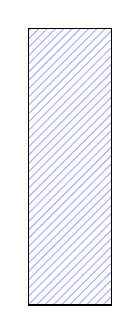
\begin{tikzpicture}
%		\node [mlp] (mlp1) {$MLP_{enc}$};
		\node [dec_z] (e1) {};
	\end{tikzpicture}
\end{center}
\end{frame}
\end{document}